\section{Описание проекта}
\subsection{Разработка дизайна}
Так как я не дизайнер, то мне нужно оперировать концептами и эскизами интерфейса. Чтобы не тратить время верстку стандартный компонентов, я буду использовать Bootstrap. Там оформлены основные компоненты. Также есть встроенная сетка, которая позволяет делать адаптивный дизайн.

\subsection{Архитектура решения}
В данном решении есть два клиента (1-ый веб-приложение, а 2-ой десктоп), один веб-сервер (он обслуживает оба клиента) и СУБД \textcite{postgres}.

\begin{figure}[H]
    \begin{center}
        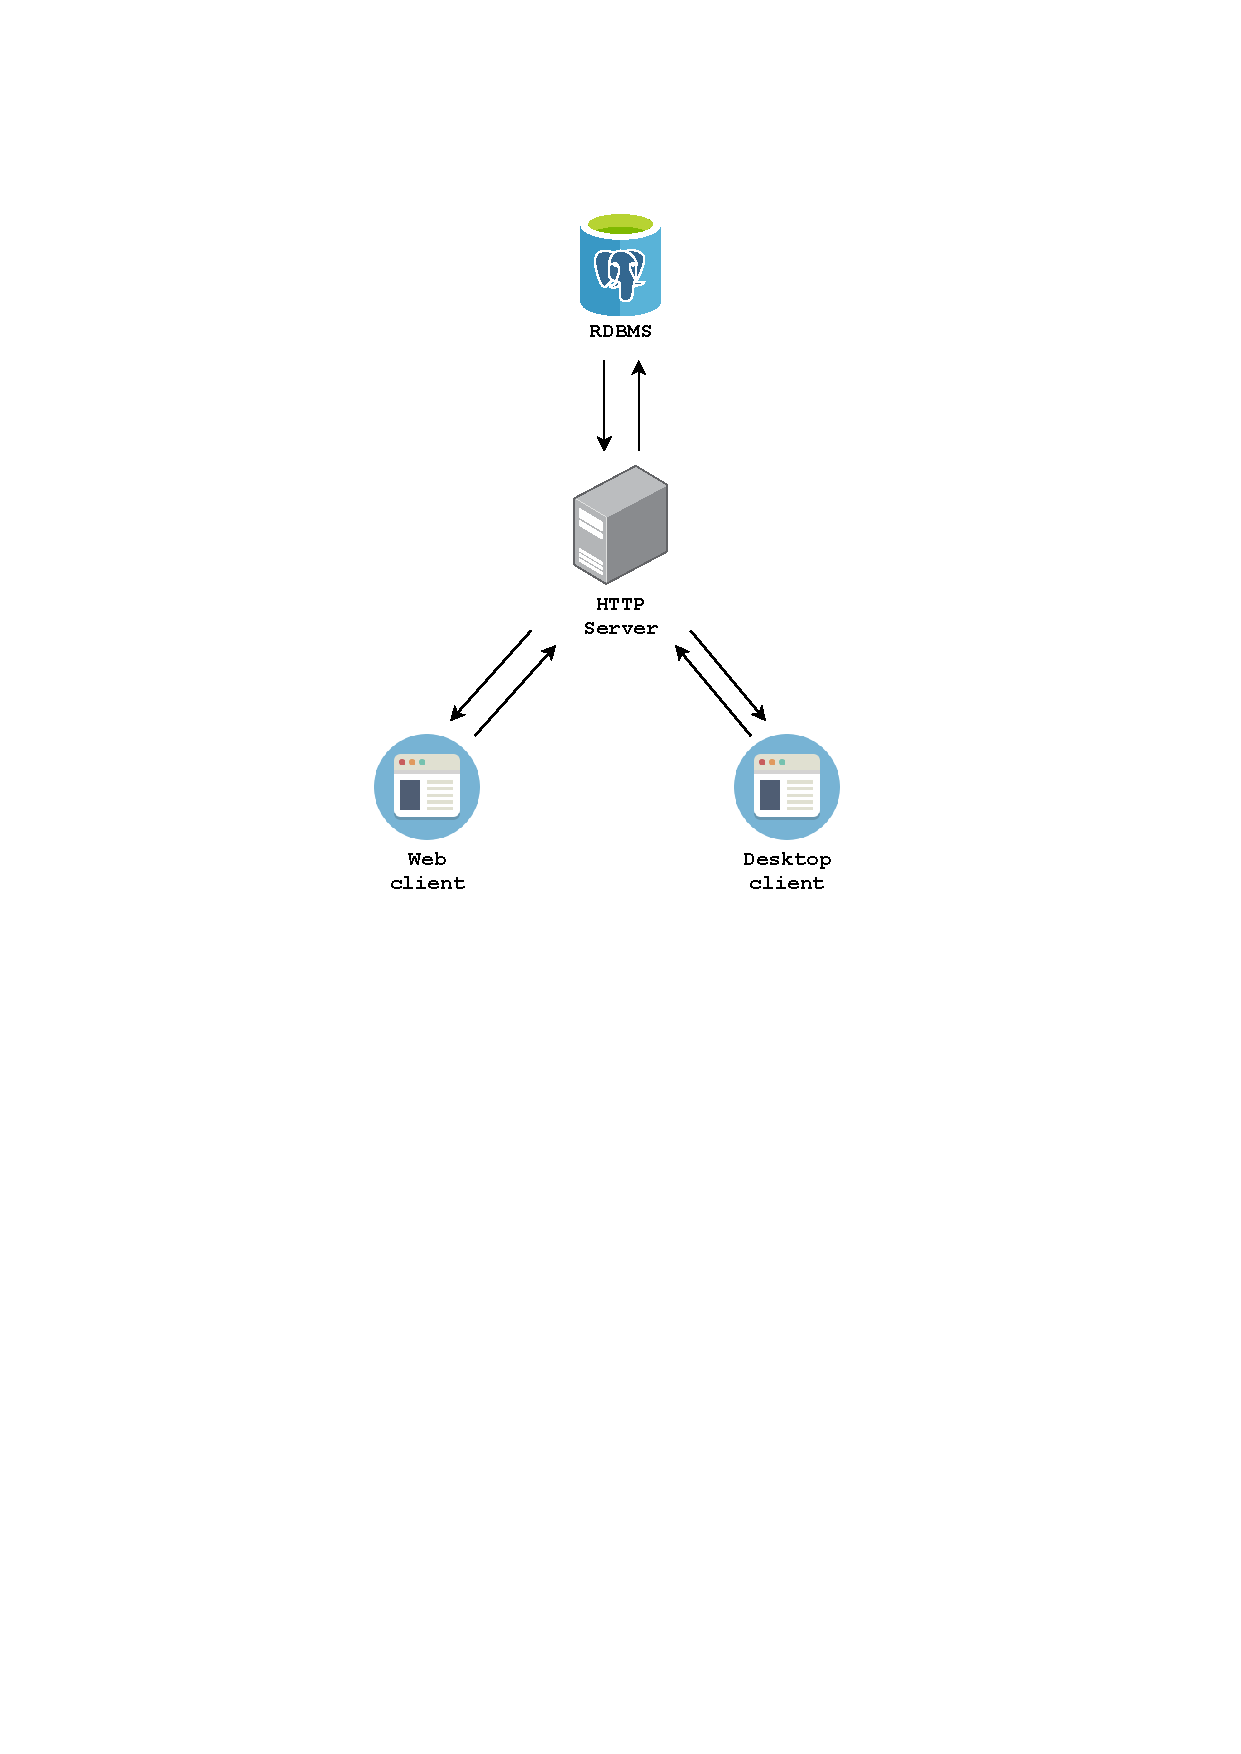
\includegraphics[trim=100 400 100 100,clip,scale=0.7]{images/app_scheme.pdf}
    \end{center}
    \caption{Схема архитектуры решения}
\end{figure}

Так как десктоп приложение работает на Electron, то необходимо на сервере обработать отправку нужного шаблона. Для этого есть проверка заголовка \mintinline{text}{User-agent} в главном роуторе:

\begin{pycode}
path = f"{PROJECT_PATH}/src/routes/main.js"

print(r"\inputminted{js}{" + path + r"}")
\end{pycode}
\captionof{listing}{Исходный код главного роутора}

\subsection{Авторизация через \acrfull{jwt}}

\subsubsection{Авторизация}
\textbf{Авторизация} --- это процесс предоставления определённому лицу или группе лиц прав на выполнение определённых действий. Также сюда входит проверка данных, прав при попытке выполнения этих действий.

\subsubsection{Аутентификация}
\textbf{Аутентификация} --- процедура проверки подлинности данный.

\subsubsection{\acrfull{jwt}}
\begin{figure}[h!]
    \begin{center}
        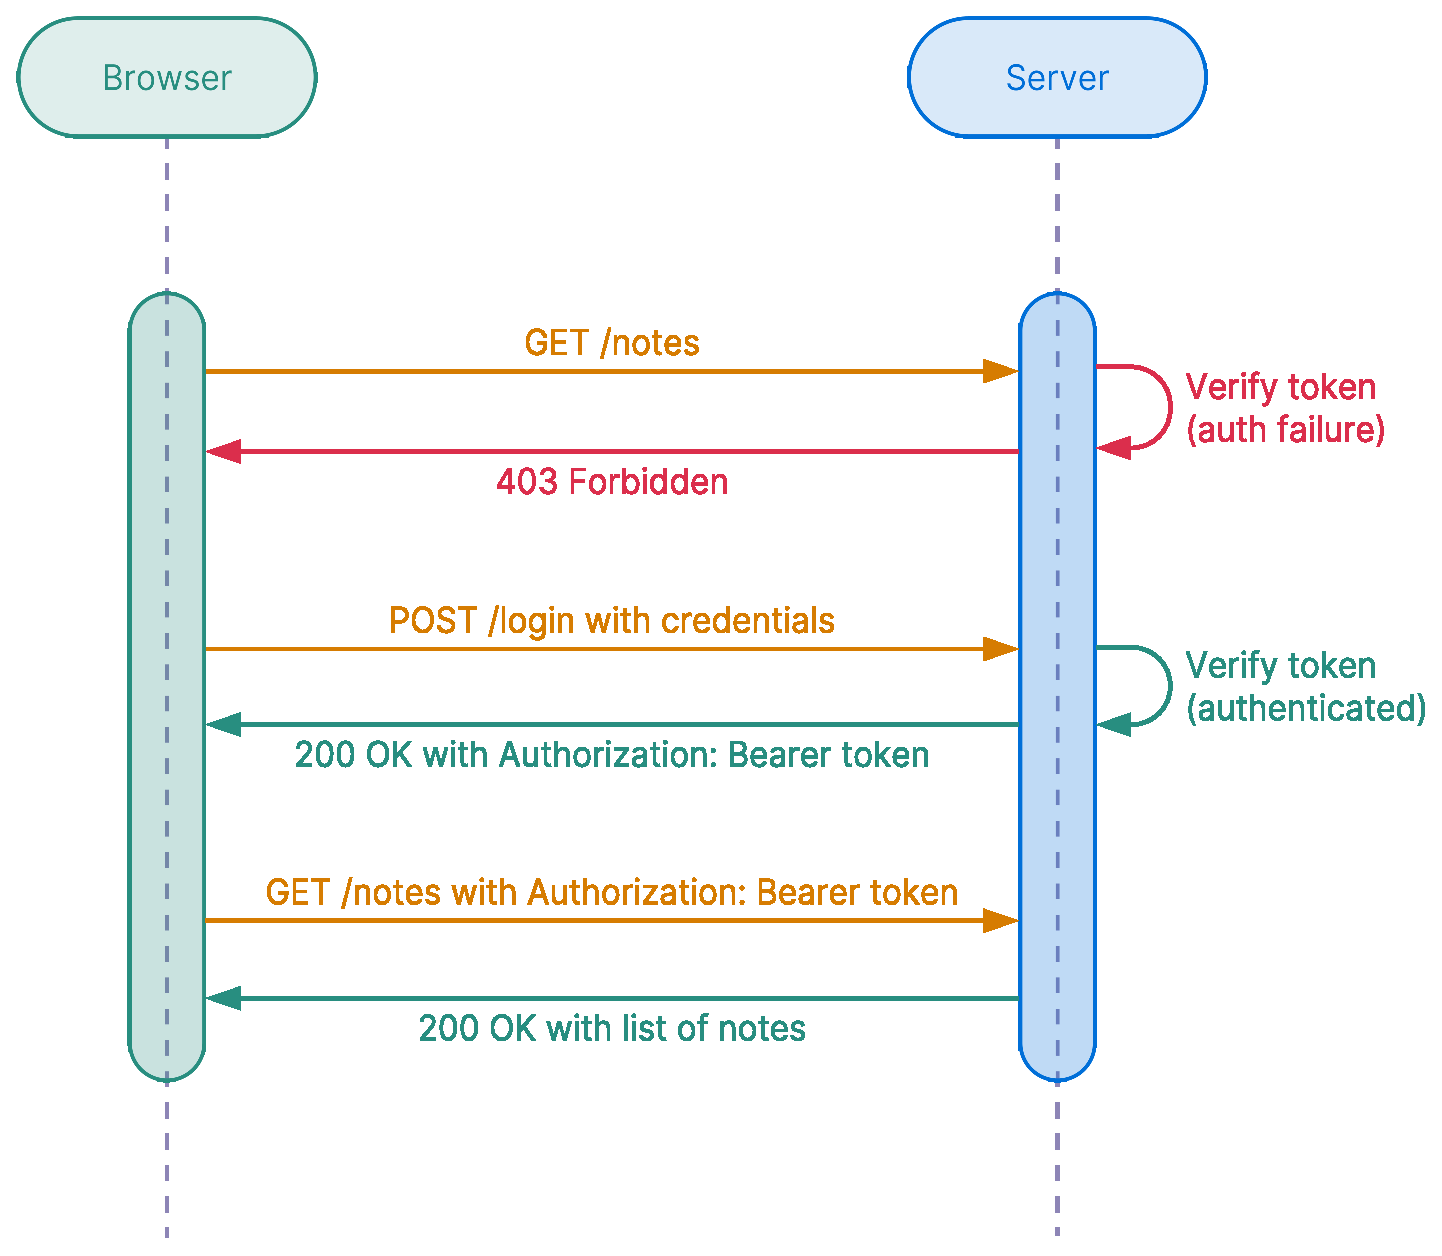
\includegraphics[scale=0.4]{images/jwt-example.eps}
        \caption{Демонстрация работы \acrshort{jwt}}
    \end{center}
\end{figure}

\textbf{\acrfull{jwt}} --- это открытый стандарт \href{https://tools.ietf.org/html/rfc7519}{(RFC 7519)}, который определяет способ для безопасной передачи информации между сторонами с помощью \acrshort{json} объектов. Эту информацию можно проверить, потому что она имеет цифровую подпись.

Вот несколько сценариев, в которых полезен \acrshort{jwt}:
\begin{itemize}
    \item \textbf{Авторизация} --- это наиболее распространенный сценарий использования \acrshort{jwt}. После того, как пользователь вошел в систему, каждый последующий запрос будет включать \acrshort{jwt}, позволяя пользователю получать доступ к маршрутам, службам и ресурсам, разрешенным с помощью этого токена.
    \item \textbf{Обмен информацией} --- \acrshort{jwt} хороший способ безопасной передачи информации между сторонами. Поскольку \acrshort{jwt} могут быть подписаны, например, с использованием пар открытого и закрытого ключей, вы можете быть уверены, что отправители являются теми, кем они себя называют. Кроме того, поскольку подпись рассчитывается с использованием \textbf{заголовка} и \textbf{полезных данных}, вы также можете убедиться, что содержимое не было изменено.
\end{itemize}

\acrshort{jwt} состоит из следующих частей:
\begin{itemize}
    \item \textbf{Заголовок} --- содержит информацию о том, как должна вычисляться подпись. Обычно состоит из двух частей: типа токена, которым является \acrshort{jwt}, и используемого алгоритма подписи, такого как HMAC SHA256 или RSA.
    \item \textbf{Полезные данные} --- это данные, которые хранятся внутри \acrshort{jwt}. Они также называют JWT-claims (заявки). Список доступных полей для \acrshort{jwt} доступен на \href{https://en.wikipedia.org/wiki/JSON_Web_Token#Standard_fields}{Wiki}.
    \item \textbf{Подпись} --- используется для проверки того, что сообщение не было изменено в процессе. В компактной форме \acrshort{jwt} является сторой, которая состоит из трех частей, разделенных точками. Псевдокод вычисления подписи:
    \begin{noerr}
    \begin{minted}{js}
SECRET_KEY = 'some string';
unsignedToken = encodeBase64Url(header) + '.' + encodeBase64Url(payload)
signature = SHA256(unsignedToken, SECRET_KEY);

// собираем всё вместе
jwt = encodeBase64Url(header) + '.' + encodeBase64Url(payload) + '.' + encodeBase64Url(signature);
    \end{minted}
    \end{noerr}
\end{itemize}

\subsubsection{Реализация}
Авторизация проходит следущим образом:
\begin{enumerate}
    \item Пользователь делает \mintinline{text}{POST /api/signup} запрос на регистрацию. Если всё нормально, то в базе данных создаётся запись с данными пользователя.
    \item Пользователь делает \mintinline{text}{POST /api/signin} запрос на аутентификацию. Если данные верные, то высылается \acrshort{jwt} вместе с состоянием пользователя (логин, почта). Когда ответ с сервера получен, то \acrshort{jwt} сохраняется в \mintinline{text}{localStorage} (долговременное хранилище), а состояние передается в глобальное \textcite{redux} хранилище.
    \item После того, как состояние глобального хранилища обновилось, приложение обновляет интерфейс.
\end{enumerate}

Если перезагрузить веб-страницу, то \textcite{redux} хранилище обнуляется. Поэтому нам нужно сделать следующее: при запуске приложения проверять на валидность JWT, который лежит в \mintinline{text}{localStorage}. Это делается через \mintinline{text}{POST /api/init} запрос. Если токен валидный, то переавторизовываем пользователя. Иначе перенаправляем на главную страницу.

Далее этот токет будет использоваться для доступа к защищёнными ресурсам. Для проверки доступа к ресурсу была реализована middleware, которая исполняется перед основным обработчиком запроса. Если токен валидный, то запрос идёт дальше c извлечёнными данными из \acrshort{jwt}, иначе сервер отвечает со статусом \mintinline{text}{403 Forbidden}.

\begin{pycode}
path = f"{PROJECT_PATH}/src/middlewares/checkToken.js"

print(r"\inputminted{js}{" + path + r"}")
\end{pycode}
\captionof{listing}{Исходный код middleware checkToken.js}

\subsubsection{Ограничение доступа к страницам}
Для ограничения доступа к определенным страницам я сделал high-order компоненты: \mintinline{text}{PrivateRoute}, \mintinline{text}{NotIsLoggedInRoute}.

\mintinline{text}{PrivateRoute} -- нужен для ограничения доступа к страницам, где нужна авторизация.

\begin{pycode}
path = f"{PROJECT_PATH}/src/client/hoc/PrivateRoute/PrivateRoute.jsx"

print(r"\inputminted{jsx}{" + path + r"}")
\end{pycode}
\captionof{listing}{Исходный код PrivateRoute.jsx}

\mintinline{text}{NotIsLoggedInRoute} -- нужен для ограничения доступа к страницам, где не нужна авторизация.

\begin{pycode}
path = f"{PROJECT_PATH}/src/client/hoc/NotIsLoggedInRoute/NotIsLoggedInRoute.jsx"

print(r"\inputminted{jsx}{" + path + r"}")
\end{pycode}
\captionof{listing}{Исходный код NotIsLoggedInRoute.jsx}

Оба компонента являются обёрткой над \mintinline{text}{Route} из библиотеки \mintinline{text}{react-router-dom}.

\subsection{API сервера}
\begin{itemize}
    \item Пользователь: \begin{itemize}
        \item \mintinline{text}{POST /api/profile/delete} -- удаление пользователя.
        \item \mintinline{text}{POST /api/profile/update-password} -- обновление пароля пользователя.
        \item \mintinline{text}{POST /api/signup} -- регистрация пользователя.
        \item \mintinline{text}{POST /api/signin} -- аутентификация пользователя.
    \end{itemize}
    \item Тест: \begin{itemize}
        \item \mintinline{text}{POST /api/test/create} -- создание теста.
        \item \mintinline{text}{PUT /api/test/update} -- обновление теста.
        \item \mintinline{text}{POST /api/test/update} -- получение теста для редактирования.
        \item \mintinline{text}{GET /api/test/pass} -- получение теста для прохождения.
        \item \mintinline{text}{GET /api/test/result} -- получение результа попытки.
        \item \mintinline{text}{POST /api/test/check} -- проверка ответов теста.
        \item \mintinline{text}{GET /api/test/profile} -- получение собственных тестов.
        \item \mintinline{text}{GET /api/test/all} -- получение всех тестов.
        \item \mintinline{text}{DELETE /api/test/delete} -- удаление теста.
    \end{itemize}
    \item Попытка: \begin{itemize}
        \item \mintinline{text}{GET /api/attempt/test} -- получение статистики теста.
        \item \mintinline{text}{GET /api/attempt/profile} -- получение попыток пользователя.
    \end{itemize}
\end{itemize}

\subsubsection{Обработка ошибок}
Если во время обработки запроса появилась ошибка, то она идёт в middleware \mintinline{text}{errorHandler}. Там формируется ответ с кодом ошибки и с сообщениями.

\begin{pycode}
path = f"{PROJECT_PATH}/src/middlewares/errorHandler.js"

print(r"\inputminted{js}{" + path + r"}")
\end{pycode}
\captionof{listing}{Исходный код middleware errorHandler.js}

\subsection{Схема базы данных}
\begin{figure}[h!]
    \begin{center}
        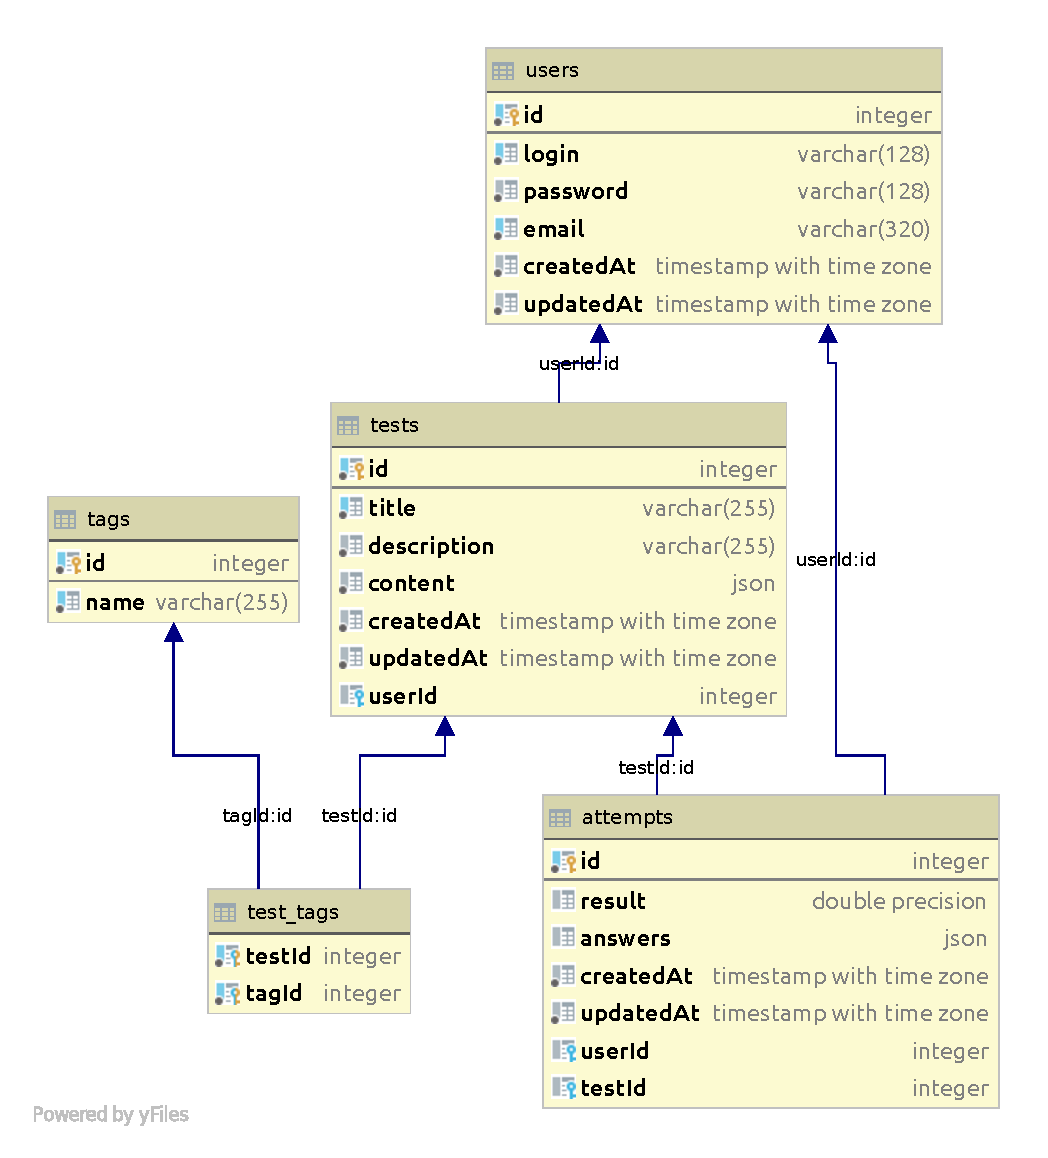
\includegraphics[scale=0.6]{images/db_scheme.eps}
    \end{center}
    \caption{Схема базы данных}
\end{figure}

\subsubsection{Связи}
\begin{itemize}
    \item (users) $1:N$ (tests)
    \item (tests) $M:N$ (tags)
    \item (attempts) $1:1$ (tests)
    \item (attempts) $1:1$ (users)
\end{itemize}
\paragraph{Примечание:}

\begin{itemize}
    \item $1:N$ -- один ко многим
    \item $M:N$ -- многие ко многим
    \item $1:1$ -- один к одному
\end{itemize}

\subsubsection{Хуки (Триггеры)}
Для некоторых таблиц заданы хуки, которые позволяют обработать события связанные с вставкой, обновлением, удалением и т.д.

\begin{itemize}
    \item \mintinline{ts}{User}: \begin{itemize}
        \item \mintinline{ts}{beforeCreate} -- шифрует пароль перед вставкой в таблицу.
        \item \mintinline{ts}{beforeUpdate} -- шифрует пароль перед обновлением.
    \end{itemize}
    \item \mintinline{ts}{Attempt}: \begin{itemize}
        \item \mintinline{ts}{afterUpdate} -- удаляет все попытки у теста, если он был изменён.
    \end{itemize}
    \item \mintinline{ts}{TestTag}: \begin{itemize}
        \item \mintinline{ts}{afterDelete} -- удаляет теги, которое не используются.
    \end{itemize}
\end{itemize}

\subsubsection{Процедуры (методы модели)}
Для модели \mintinline{ts}{User} есть две процедуры:
\begin{itemize}
    \item \mintinline{ts}{comparePasswords(password: string)} -- инстанс метод, который стравнивает пароль текущего пользователя с \mintinline{ts}{password}.
    \item \mintinline{ts}{hashPassword(password: string)} -- статический метод, который шифрует \mintinline{ts}{password}.
\end{itemize}

\subsubsection{Каскадное удаление}
Каскадное удаление в мире реляционных баз данных позволяет удалять связанные данные из зависимой таблицы, при удалении данных из основной таблицы. У меня оно использую во всех таблицах.

\clearpage